%\documentclass{beamer} 
\documentclass[handout]{beamer} % sin pausas
\usetheme{CambridgeUS}

\usepackage[utf8]{inputenc}%esto permite (en Windows) escribir directamente 
\usepackage{graphicx}
\usepackage{array}
\usepackage{tikz} 
\usetikzlibrary{shapes,arrows,babel,decorations.pathreplacing}
\usepackage{verbatim} 
\usepackage{xcolor} 
\usepackage{amsgen,amsmath,amstext,amsbsy,amsopn,amsfonts,amssymb}
\usepackage{amsthm}
\usepackage{tikz}
\usepackage{tkz-graph}
\usepackage{mathtools}
\usepackage{xcolor}

%\setbeamertemplate{background}[grid][step=8 ]
\setbeamertemplate{itemize item}{$\circ$}
\setbeamertemplate{enumerate items}[default]

\definecolor{links}{HTML}{2A1B81}
\hypersetup{colorlinks,linkcolor=,urlcolor=links}

\newcommand{\img}{\operatorname{Im}}
\newcommand{\nuc}{\operatorname{Nu}}
\newcommand\im{\operatorname{Im}}
\renewcommand\nu{\operatorname{Nu}}
\newcommand{\la}{\langle}
\newcommand{\ra}{\rangle}
\renewcommand{\t}{{\operatorname{t}}}
\renewcommand{\sin}{{\,\operatorname{sen}}}
\newcommand{\Q}{\mathbb Q}
\newcommand{\R}{\mathbb R}
\newcommand{\C}{\mathbb C}
\newcommand{\K}{\mathbb K}
\newcommand{\F}{\mathbb F}
\newcommand{\Z}{\mathbb Z}

\renewcommand{\figurename }{Figura}
%\usepackage{enumitem}
%\setlist[itemize]{itemsep=10pt, label={$\circ$}}
%\newtheorem{teorema}{Teorema}
%\newtheorem{corolario}[teorema]{Corolario}
%\newtheorem{proposicion}[teorema]{Proposición}

%\theoremstyle{definition}
%\newtheorem{definicion}[theorem]{Definici\'on}
%\newtheorem{ejemplo}[theorem]{Ejemplo}
%\newtheorem{pregunta}[equation]{Pregunta}
%\newtheorem{step}{Paso}



\newenvironment{exercise}[1]% environment name
{% begin code
	\par\vspace{\baselineskip}\noindent
	\textbf{Ejercicio (#1)}\begin{itshape}%
		\par\vspace{\baselineskip}\noindent\ignorespaces
	}%
	{% end code
	\end{itshape}\ignorespacesafterend
}


\newenvironment{definicion}% environment name
{% begin code
	\par\vskip .2cm%
	{\color{blue}Definición}%
	\vskip .2cm
}%
{%
	\vskip .2cm}% end code

\newenvironment{observacion}% environment name
{% begin code
	\par\vskip .2cm%
	{\color{blue}Observación}%
	\vskip .2cm
}%
{%
	\vskip .2cm}% end code

\newenvironment{ejemplo}% environment name
{% begin code
	\par\vskip .2cm%
	{\color{blue}Ejemplo}%
	\vskip .2cm
}%
{%
	\vskip .2cm}% end code

\newenvironment{ejercicio}% environment name
{% begin code
	\par\vskip .2cm%
	{\color{blue}Ejercicio}%
	\vskip .2cm
}%
{%
	\vskip .2cm}% end code


\renewenvironment{proof}% environment name
{% begin code
	\par\vskip .2cm%
	{\color{blue}Demostración}%
	\vskip .2cm
}%
{%
	\vskip .2cm}% end code



\newenvironment{demostracion}% environment name
{% begin code
	\par\vskip .2cm%
	{\color{blue}Demostración}%
	\vskip .2cm
}%
{%
	\vskip .2cm}% end code

\newenvironment{idea}% environment name
{% begin code
	\par\vskip .2cm%
	{\color{blue}Idea de la demostración}%
	\vskip .2cm
}%
{%
	\vskip .2cm}% end code

\newenvironment{solucion}% environment name
{% begin code
	\par\vskip .2cm%
	{\color{blue}Solución}%
	\vskip .2cm
}%
{%
	\vskip .2cm}% end code



\newenvironment{lema}% environment name
{% begin code
	\par\vskip .2cm%
	{\color{blue}Lema}\begin{itshape}%
		\par\vskip .2cm
	}%
	{% end code
	\end{itshape}\vskip .2cm\ignorespacesafterend
}

\newenvironment{proposicion}% environment name
{% begin code
	\par\vskip .2cm%
	{\color{blue}Proposición}\begin{itshape}%
		\par\vskip .2cm
	}%
	{% end code
	\end{itshape}\vskip .2cm\ignorespacesafterend
}

\newenvironment{teorema}% environment name
{% begin code
	\par\vskip .2cm%
	{\color{blue}Teorema}\begin{itshape}%
		\par\vskip .2cm
	}%
	{% end code
	\end{itshape}\vskip .2cm\ignorespacesafterend
}


\newenvironment{corolario}% environment name
{% begin code
	\par\vskip .2cm%
	{\color{blue}Corolario}\begin{itshape}%
		\par\vskip .2cm
	}%
	{% end code
	\end{itshape}\vskip .2cm\ignorespacesafterend
}

\newenvironment{propiedad}% environment name
{% begin code
	\par\vskip .2cm%
	{\color{blue}Propiedad}\begin{itshape}%
		\par\vskip .2cm
	}%
	{% end code
	\end{itshape}\vskip .2cm\ignorespacesafterend
}




\title[Clase 1 - Números  complejos]{Álgebra/Álgebra II \\ Clase 1 - Números complejos}
%\author[C. Olmos / A. Tiraboschi]{Carlos Olmos / Alejandro Tiraboschi}
\institute[]{\normalsize FAMAF / UNC
	\\[\baselineskip] ${}^{}$
	\\[\baselineskip]
}
\date[25/08/2020]{25 de agosto de 2020}




\begin{document}
	
	\frame{\titlepage} 
	
\begin{frame}{Introducci\'on}
	
	En esta clase introduciremos el conjunto $\mathbb{C}$ de n\'umeros complejos junto a sus operaciones de suma y multiplicaci\'on. Adem\'as,
	\begin{itemize}
		\item Definiremos los conceptos de ``conjugado'', ``argumento'' y ``m\'odulo'' de un n\'umero complejo;
		\item Aprenderemos a calcular el inverso de un n\'umero complejo;
		\item Veremos como representar gr\'aficamente los n\'umeros complejos;
	\end{itemize}
	
	
	\
	
	Estas diapositivas estan basadas en la secci\'on A.2 de las {\it Notas de \'Algebra II} del curso, siguiendo la misma numeraci\'on. 
	
	
\end{frame}	

\begin{frame}\frametitle{Números complejos:  definición}
	
	\vskip .4cm 
	
	
	¿La ecuación  $x^2 + 1 =0$ tiene solución?
	
	\vskip .4cm
	\pause 
	
	En $\mathbb R$ no:  $x^2 \ge 0$  y por lo tanto $x^2 + 1 >0$.
	
	\pause 
	\vskip .4cm

 Podemos extender $\mathbb R$ a otro cuerpo,  de tal forma que \textit{toda} ecuación polinómica con coeficentes en $\mathbb R$ tenga solución. 
 
 \pause
 \vskip .4cm
	
	\begin{definicion} 
		Los \textit{números complejos}\index{números complejos} es el conjunto $\mathbb C$  de los pares ordendados $(a,b)$,  denotados $a+ib$, con $a, b$  en $\mathbb R$, con las operaciones '$+$' y '$\cdot$', definidas
		\begin{align}
		(a+ib)+ (c+id) &:= (a+c) + i(b+d), \label{sumacompleja} \\
		(a+ib) \cdot (c+id) &:= (ac -bd) + i(ad+bc). \label{productocomplejo}
		\end{align}
	
	\end{definicion}
	
\end{frame}

\begin{frame}
	\begin{itemize}
		
		
		\item	La definición de la suma de dos números complejos es ``coordenada a coordenada''. 
		\pause
		\vskip .3cm
		\item		Por la definición de producto:
		\begin{equation*}
		i^2 = (0 + i\cdot 1)(0 + i\cdot 1) = (0\cdot 0 - 1 \cdot 1) + i(0\cdot 1 + 1 \cdot 0) = -1.
		\end{equation*} 
		Luego, $i^2 = -1$ e  $i$  es la solución de la ecuación polinómica $x^2 + 1 =0$.
		\pause	\vskip .3cm
		
		\item Sabiendo  que $i^2 = -1$ y la propiedad distributiva, no necesitamos memorizar la fórmula del producto:
		\begin{align*}
		(a+ ib)(c+ id) &= ac + iad + i bc + i^2 bd \\
		&=  ac + iad + i bc - bd\\
		&= (ac-bc) + i(ad+bc).
		\end{align*}
	\end{itemize}
\end{frame}

\begin{frame}
	
	\begin{itemize}
	
	
		\item Al número complejo $i = 0 + i\cdot 1$ lo llamamos el \textit{imaginario puro}.  
			
		\vskip .4cm\pause
		
		\item Si $z= a + ib$  es un número complejo,  diremos que $a$ es la \textit{parte real} de $z$ y  la denotamos $a =  \frak{Re}\, z$. Por otro lado,  $b$ es la \textit{parte  imaginaria} de $z$ que es denotada $b = \frak{Im}\, z$.
		
		\vskip .4cm\pause
		\item Es claro  que 
		\begin{equation*}
		a+ bi = c+ di\quad \Leftrightarrow\quad a=c \;\wedge\; b = d.
		\end{equation*}
		
		\vskip .4cm\pause
		
		\item $\R \subseteq\C$,  con la correspondencia $a \to a + i \cdot 0$ y  observamos que si  nos restringimos a $\R$, tenemos las reglas de adición y  multiplicación usuales.  
\end{itemize}	
\end{frame}


\begin{frame}
	Con la definición de suma y producto  los  números complejos forman  un  \textit{anillo conmutativo  con  1}. 
	
	\vskip .3cm\pause
	
	Es decir,  cumplen todas las propiedades de los números enteros,  salvo las de orden. 
	
		\vskip .3cm\pause
		
		
	En particular la suma y el producto son conmutativos, asociativos,  se cumplen las  propiedades distributivas, etc. 
	
		\vskip .3cm\pause
		
	Más aún,  como veremos más adelante,  $\mathbb C$  es un cuerpo (como lo es $\mathbb R$): es decir todo número complejo  no nulo tiene un inverso multiplicativo. \vskip .3cm\pause Simbólicamente
	\begin{equation*}
		z \ne 0 \quad \Rightarrow \quad \exists w \text{ tal que } zw = 1.
	\end{equation*} 
	($w$  se denota $z^{-1}$).
\end{frame}

\begin{frame}
	\begin{itemize}
	
	
	\item	La definición de la suma de dos números complejos es ``coordenada a coordenada''. 
		\pause
				\vskip .3cm
				

	
	\item	$0 = 0 + i\cdot 0\in \C$,   es el elemento neutro de la suma. 
	\begin{equation*}
		(a + ib) + (0 + i\cdot 0 ) = (a +0) +  i\cdot(b+0)  = a +  i\cdot b.
	\end{equation*}
	
	\pause		\vskip .3cm
	\item	Si $z = a + ib$,  entonces $-z = -a -ib$ es el opuesto aditivo de $z$. 
		\begin{equation*}
	(a + ib) + (-a - i\cdot b ) = (a -a ) +  i\cdot(b-b)  = 0 +  i\cdot 0.
	\end{equation*}
	
		\pause		\vskip .3cm
	
	\item	$1 = 1 + i\cdot 0 \in \C$,   es el elemento neutro del producto. 
\end{itemize}
\end{frame}


\begin{frame}\frametitle{Representación gráfica de los números complejos}
	
		Hemos definido los números complejos como pares ordenados y como tales es posible representarlos en el plano $\R \times \R$:	

\begin{center}
	\begin{tikzpicture}[scale=0.8]
	\draw[->] (-1.0,0) -- (4.0,0) node[right] {}; % eje x
	\draw[->] (0,-1) -- (0,3) node[above] {}; % eje y
	\draw[fill] (2.5,1.5) circle [radius=0.05];
	\node [right] at (2.5,1.5) {$a+ ib$};
	\node [below] at (2.5,-3pt) {$a$};
	\node [left] at (-3pt,1.5) {$b$};
	\draw (2.5,-3pt) -- (2.5,3pt);
	\draw (-3pt, 1.5) -- (3pt, 1.5);
	\draw [dashed] (0,1.5) -- (2.5,1.5);
	\draw [dashed] (2.5,0) -- (2.5,1.5);
	\end{tikzpicture}
\end{center}

\end{frame}

\begin{frame}
	
	Representemos gráficamente los números $2 + i$, $-1 + i\, 2.5$ y $-2.5 -i\, 2.5$:
		\pause
	\begin{figure}[h]
		\begin{tikzpicture}
		\draw[->] (-4.0,0) -- (4.0,0) node[right] {}; % eje x
		\draw[->] (0,-3) -- (0,3) node[above] {}; % eje y
		\foreach \x in {-4,...,-1}
		\draw (\x,3pt) -- (\x,-3pt)
		node[anchor=north] {\x};
		\foreach \x in {1,...,4}
		\draw (\x,3pt) -- (\x,-3pt)
		node[anchor=north] {\x};
		\foreach \y in {-3,...,-1}
		\draw (3pt,\y) -- (-3pt,\y) 
		node[anchor=east] {\y}; 
		\foreach \y in {1,...,3}
		\draw (3pt,\y) -- (-3pt,\y) 
		node[anchor=east] {\y}; 
		\draw[fill] (2,1) circle [radius=0.05];
		\node [right] at (2,1) {$2+ i$};
		\draw [dashed] (0,1) -- (2,1);
		\draw [dashed] (2,0) -- (2,1);
		\draw[fill] (-1,2.5) circle [radius=0.05];
		\node [left] at (-1,2.5) {$-1+i \,2.5$};
		\draw [dashed] (0,2.5) -- (-1,2.5);
		\draw [dashed] (-1,0) -- (-1,2.5);
		\draw[fill] (-2.5,-2.5) circle [radius=0.05];
		\node [below] at (-2.5,-2.5) {$-2.5-i\,2.5$};
		\draw [dashed] (0,-2.5) -- (-2.5,-2.5);
		\draw [dashed] (-2.5,0) -- (-2.5,-2.5);
		\end{tikzpicture}
		\end{figure}	
\end{frame}

\begin{frame}
		Con esta representación gráfica la definición de la suma de dos números complejos es la suma ``coordenada a coordenada''. 
		
		\vskip .3cm \pause
		Ejemplificamos la suma de números complejos en el plano: 
	
		\begin{figure}[h]
		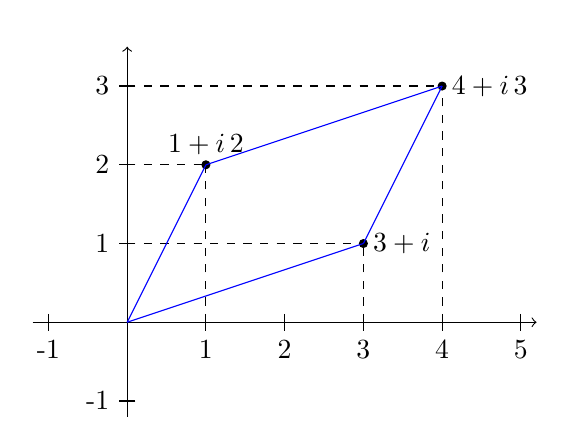
\begin{tikzpicture}
		\def\px{3.0}
		\def\py{1.0}
		\def\qx{1.0}
		\def\qy{2.0}
		\draw[->] (-1.2,0) -- (5.2,0) node[right] {}; % eje x
		\draw[->] (0,-1.2) -- (0,3.5) node[above] {}; % eje y
		\foreach \x in {-1}
		\draw (\x,3pt) -- (\x,-3pt)
		node[anchor=north] {\x};
		\foreach \x in {1,...,5}
		\draw (\x,3pt) -- (\x,-3pt)
		node[anchor=north] {\x};
		\foreach \y in {-1}
		\draw (3pt,\y) -- (-3pt,\y) 
		node[anchor=east] {\y}; 
		\foreach \y in {1,...,3}
		\draw (3pt,\y) -- (-3pt,\y) 
		node[anchor=east] {\y}; 
		\draw[fill] (\px,\py) circle [radius=0.05];
		\node [right] at (\px,\py) {$3+ i$};
		\draw [dashed] (0,\py) -- (\px,\py);
		\draw [dashed] (\px,0) -- (\px,\py);
		\draw[fill] (\qx,\qy) circle [radius=0.05];
		\node [above] at (\qx,\qy) {$1+i \,2$};
		\draw [dashed] (0,\qy) -- (\qx,\qy);
		\draw [dashed] (\qx,0) -- (\qx,\qy);
		\draw[fill] (\qx +\px, \qy + \py) circle [radius=0.05];
		\node [right] at (\qx+\px,\qy + \py) {$4+i\,3$};
		\draw [dashed] (0, \qy + \py) -- (\qx+\px,\qy + \py);
		\draw [dashed] (\qx+\px,0) -- (\qx+\px, \qy+ \py);
		\draw[-,blue] (0,0) -- (\qx,\qy);
		\draw[-,blue] (0,0) -- (\px,\py);
		\draw[-,blue] (\qx,\qy) -- (\qx+\px, \qy + \py);
		\draw[-,blue] (\px,\py) -- (\qx+\px, \qy + \py);
		\end{tikzpicture}
	\end{figure}
\end{frame}


\begin{frame}\frametitle{Módulo y conjugado  de un número complejo}
			
	\begin{definicion} Sea $z = a + ib \in \C$. 
		\vskip .3cm \pause
		\begin{itemize}
			\item El \textit{módulo} de $z$ es \qquad $|z| = \sqrt{a^2+b^2}$.
			\vskip .3cm \pause
			\item  El  \textit{conjugado} de $z$ es \quad $\bar z = a-ib$.
		\end{itemize}
	\pause
	\end{definicion} 
\vskip -0.3cm
			\begin{figure}[h]
		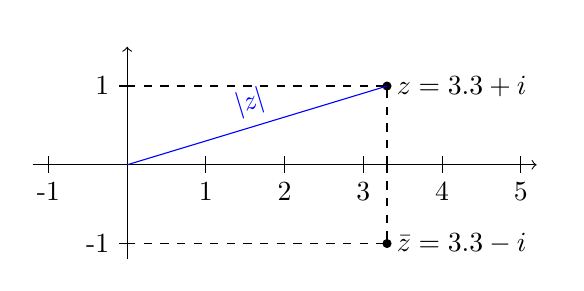
\begin{tikzpicture}
		\def\px{3.3}
		\def\py{1.0}
		\def\qx{3.3}
		\def\qy{-1.0}
		\draw[->] (-1.2,0) -- (5.2,0) node[right] {}; % eje x
		\draw[->] (0,-1.2) -- (0,1.5) node[above] {}; % eje y
		\foreach \x in {-1}
		\draw (\x,3pt) -- (\x,-3pt)
		node[anchor=north] {\x};
		\foreach \x in {1,...,5}
		\draw (\x,3pt) -- (\x,-3pt)
		node[anchor=north] {\x};
		\foreach \y in {-1}
		\draw (3pt,\y) -- (-3pt,\y) 
		node[anchor=east] {\y}; 
		\foreach \y in {1}
		\draw (3pt,\y) -- (-3pt,\y) 
		node[anchor=east] {\y}; 
		\draw[fill] (\px,\py) circle [radius=0.05];
		\node [right] at (\px,\py) {$z= \px + i$};
		\draw [dashed] (0,\py) -- (\px,\py);
		\draw [dashed] (\px,0) -- (\px,\py);
		\draw[fill] (\qx,\qy) circle [radius=0.05];
		\node [right] at (\qx,\qy) {$\bar z = \qx- i$};
		\draw [dashed] (0,\qy) -- (\qx,\qy);
		\draw [dashed] (\qx,0) -- (\qx,\qy);
		\draw[-,blue]  (0,0)  -- (\px,\py)  node[midway, above, sloped] {$|z|$};
		%\draw[-,blue] (0,0) -- (\px,\py)node[above] {$|z|$};
		\end{tikzpicture}
	\end{figure}
	
\end{frame}

\begin{frame}
		\begin{proposicion} Sean $z$ y $w$ números complejos. Entonces, \vskip .3cm
		\begin{enumerate}
			\item $|z| =0 \Leftrightarrow z=0$.\vskip .3cm\pause
			\item $z\bar{z} = |z|^2$.\vskip .3cm\pause
			\item  $\overline{z+w} = \overline{z} + \overline{w}$.\vskip .3cm\pause
			\item  $\overline{zw} = \overline{z}\;  \overline{w}$.\vskip .3cm\pause
		\end{enumerate}
	\end{proposicion}



		\begin{proof}

1. Si $z = a +ib$, 
\begin{align*}
|z| =0 &\Leftrightarrow \sqrt{a^2+b^2}  \Leftrightarrow {a^2+b^2} \Leftrightarrow {a^2 =0 \wedge b^2 =0}\\
&\Leftrightarrow {a =0 \wedge b =0} \Leftrightarrow z=0.
\end{align*}




\end{proof}	
\end{frame}

\begin{frame}
		2. Si  $z = a + ib$, entonces $\bar z = a -ib$, y
	\begin{equation*}
	z\bar{z} =(a + ib)( a -ib) = a^2 + iab -iba -i^2 b^2 =  a^2 -(-1) b^2 =  a^2  +  b^2.
	\end{equation*}
	
	\pause  \vskip .4cm 
	3. 		Si $z = a + i b$ y $w = c +i d$, entonces
	\begin{align*}
	\overline{z+w} &=  \overline{(a+c) + i(b+d)} = (a+c) - i(b+d), \\
	\overline{z} + \overline{w} &= a - i b + c -i d =  (a+c) - i(b+d).
	\end{align*}
	Por lo tanto $	\overline{z+w} = \overline{z}+\overline{w}$. 
	\pause  \vskip .4cm 
	4. 	Si $z = a + ib$ y $w = c +id$, entonces 
	\begin{align*}
	\overline{zw} &= \overline{(a+ib) (c+id) } = \overline{(ac -bd) + i(ad+bc) }= (ac -bd) - i(ad+bc), \\
		\overline{z}\;  \overline{w} &=(a - ib)(c-id) = (ac -bd) - i(ad+bc).
	\end{align*} 
	Por lo tanto $	\overline{zw} = \overline{z}\;  \overline{w}$. \qed
	
	
\end{frame}
\begin{frame}\frametitle{Inverso de  un número complejo}
	
	\begin{proposicion} Sea $z$  un número complejo no  nulo. Entonces,  $z^{-1} = \displaystyle\frac{\overline{z}}{|z|^2}$.

\end{proposicion}\pause  \vskip .4cm 
	\begin{proof}\pause 
		Ya vimos que  $z\bar{z} = |z|^2$. Como $z \ne 0$, tenemos que $|z| \ne 0$, luego 
		\begin{equation*}
			z\frac{\bar{z} }{|z|^2} = \frac{z\bar{z} }{|z|^2} =\frac{|z|^2 }{|z|^2} = 1.
		\end{equation*}
		\qed
	\end{proof}	
  \vskip 2cm 


\end{frame}


\begin{frame}
	\begin{observacion}
		Multiplicar por  un número real es ``coordenada a coordenada'', luego si $z = a + ib$, tenemos que $z^{-1} = \displaystyle\frac{{1\,\,}}{|z|^2}\,\overline{z}$, es decir
		\begin{equation*}
		(a+ ib)^{-1} = \frac{a}{a^2+b^2} -  i\frac{b}{a^2+b^2}.
		\end{equation*}
	\end{observacion}
	\pause 
	\begin{ejemplo}
		Escribir el inverso de $-1 +2i$ en la forma $a +bi$.
	\end{ejemplo}
\begin{solucion}\pause 
	Primero averiguamos el módulo al cuadrado:
	\begin{equation*}
		|-1 +2i|^2 = (-1)^2 + 2^2 = 1 + 4 = 5.
	\end{equation*}
\end{solucion}
\end{frame}


\begin{frame}
	Como $\overline{-1 +2i} = -1 - 2i$,
	\begin{equation*}
	(-1 +2i)^{-1} = -\frac{1}{5} -  i\frac{2}{5}.
	\end{equation*}
	
	\vskip .4cm
	\pause 
	Nunca está demás comprobar el resultado: 
	
	\begin{equation*}
	(-1 +2i)(-\frac{1}{5} -  i\frac{2}{5}) = \frac{1}{5}+\frac{2}{5}i - \frac{2}{5}i +\frac{4}{5} = \frac{1}{5}+ \frac{4}{5} = 1
	\end{equation*}
	\qed
\end{frame}


\begin{frame}\frametitle{Soluciones de ecuaciones polinomiales a coeficientes en $\mathbb C$}
	Extendiendo los números reales a los complejos,  encontramos un conjunto de números en donde la ecuación $x^2+1=0$ tiene solución. 
		\vskip .4cm
		\pause 
	¿Tendremos que extender $\mathbb R$ aún más para encontrar soluciones a ecuaciones polinomiales más complejas? 
	\pause 
		\vskip .4cm
	Le respuesta es: 
		\vskip .4cm
		
	{\color{blue}Teorema fundamental del álgebra} 
		\vskip .2cm
	La ecuación polinómica
		\begin{equation*}
			x^n + a_{n-1}x^{n-1} + \cdots + a_2x^2 + a_1 x + a_0 = 0,
		\end{equation*}
		con $a_i \in \mathbb C$ ($0 \le i \le n-1$) tiene solución en $\mathbb C$.
		

	
	
\end{frame}




\end{document}

